\section{Compressing an Attributed Graph}
%\begin{table}[h]
%\center\caption{Table of Symbols and Acronyms.}
%\begin{tabular}{|c|c|}
%\hline
%Symbols & Definitions\\
%\hline\hline
%$MDL$ & Minimum Description Length\\
%$IROC$ & Information-theoretic non-Redundant Overlapping Clustering\\
%\hline
%$G$ & Attributed graph\\
%$V$ & Set of vertices of a graph\\
%$E$ & Set of edges of a graph\\
%$\Lambda$ & Dimension of the attribute space \\
%$\Theta$ & Number of categories \\
%$A$ & Adjacency matrix\\
%$F$ & Attribute matrix (in some literature also called feature matrix)\\
%$C$ & Cluster in the graph\\
%$U$ & No-Cluster area, logically "unclustered"\\
%$N$ & Number of vertices \\
%$K$ & Number of Cluster \\
%$N_C$& Number of vertices in cluster $C$ \\
%$T$ & Number of all attributes, same as $|\lambda|$ for clarity reasons\\
%$\lambda_i$ & The $i$th attribute, $1<i<T$\\
%$\theta_i$ & Categories of $i$th attribute, $1<i<T$\\
%$S$ & Number of attributes of cluster $C$ \\
%$L(D|M)$ & coding costs of data D under model M \\
%$P$ & a probability, we like upper letters \\
%$ID$ & a cluster label (id)\\
%\hline
%\end{tabular}
%\label{tab:symbols}
%\end{table}
To understand our coding scheme it is foremost important to outline what needs to be compressed in an attributed graph. From start, attributed graphs are an extension from general graphs by involving attributed information to each vertex. Therefore, two types of matrices are needed to model both structural connections in the graph and the attribute space of each node. Same as the general graph, the structure is mapped into an adjacency matrix, while the attributes of each vertex can be modelled as a matrix with rows denoting vertices and columns representing attributes.  We call that matrix an \emph{attribute matrix}. So far, an attributed graph is represented by an adjacency matrix and an attributed matrix that need to be compressed for efficiency and automatization. For simplicity in this paper, we focus on undirected unweighed graphs with categorical attributes, which means both matrices are symmetric.

\subsection{Notations}

%\noindent \emph{Attributed graph} is an extension of general graph by involving attributes for each vertex, which combines relational information with descriptive information. Therefore, two matrices are adopted to represent such type of graph. Specifically, like the general graph connections between vertices are mapped as $``1"$s in an adjacency matrix, while the attributes of all vertices can be arrayed into a matrix, which is named as \emph{attribute matrix}, with rows denoting vertices and columns representing various attributes. The two matrices are related by sharing same vertices. An attribute graph $G$ is represented by an adjacency matrix $A$ and an attribute matrix $F$, which is defined in Definition \ref{def:an}. In this paper, we focus on undirected unweighed graphs with categorical attributes. 
Before we start with the coding scheme this section describes the used notation in the paper for clarification.

\begin{definition}[Attributed Graph]\label{def:an}
An attributed g-raph is defined as $G=(V,E,\Lambda)$, where $V = \{v_1, v_2,...,v_N \}$ contains $N$ vertices, $E= \{(v_i,v_j),1\leq i\leq N,1\leq j \leq N,i\neq j \}$ are edges, $\Lambda = \{\lambda_1,\lambda_2,...,\lambda_T \}$ are $T$ attributes of each vertex. $\Theta = \{\theta_1,\theta_2,...,\theta_T \}$ represents domains of $\Lambda$. $A$ is the adjacency matrix with $a_{ij}=1$ if $(v_i,v_j)\in E$ and $F$ is the attribute matrix with $f_{ik}$ denotes the categorical value of the $i$th vertex in the $k$th attribute. An attribute graph is represented as $G=(A,F)$ as well.
\end{definition}

In this paper, we aim at mining knowledge from the attributed graph by detecting non-redundant overlapping clusters. As attributed graphs possess both structural and attribute information, the cluster of such type of data covers both informations as well, which is defined in Definition \ref{def:anclus}. A cluster $C$ is a subset of an attributed graph $G$. Specifically, the cluster not only needs to be densely connected but also contains a subgroup of attributes to describe the meaning of the cluster. 
                                                            
\begin{definition}[Cluster in an Attributed Graph]\label{def:anclus}
A cluster is defined as $C =(V',E',\Lambda')$, which is a subset of the attributed graph $G$, where $V'\subseteq V$, $E'\subseteq E$, $\Lambda'\subseteq \Lambda$. $V' = \{v'_1, v'_2,...,v'_{N'} \}$ is a subset of $V$, which includes $N'$ densely connected vertices and $\Lambda' = \{\lambda'_1,\lambda'_2,...,\lambda'_S \}$ is a subset of $\Lambda$, which contains $S$ attributes with coherent categories, where $S\leq T$. $A_C \subset A$ is the subset adjacency matrix of $C$ that only contains the vertices in $C$ and $F_C \subset F$ is the subset attribute matrix of $C$. Similarly, a Cluster is represented as $C=(A_C,F_C)$.
\end{definition}

Besides the own structure of a cluster, there are some edges connecting these clusters that are not included inside the clustering. Similarly to the edge structure, many attributes from the full-dimensional subspace are not assigned to any cluster. We define these areas as the non-cluster area of an attributed graph in Definition \ref{def:nonclus}, which consists of the elements lying outside any cluster. 
                                 
\begin{definition}[Non-Cluster Area]\label{def:nonclus}
The non-cluster area of an attributed graph $G$ modelled by $K$ clusters $\{C_1$, $C_2,...,C_K \}$ is defined as $U = U_A \bigcup U_F $, where $U_A$ is the Non-Cluster area in the adjacency matrix $A$ and $U_F$ is the non-cluster area in the attributed matrix $F$. $U_A=A\setminus A'$, where $A' = A_{C_1}\cup A_{C_2}...\cup A_{C_K}$ is the combination of all structural elements appearing in $\{C_1,C_2,...,C_K \}$ and $U_F = U_{\lambda_1}\cup U_{\lambda_2}...\cup U_{\lambda_T}$, where $U_{\lambda_t}$ are entries of $F$ in attribute $\lambda_t$ which are not included in $\{C_1,C_2,...,C_K \}$.
\end{definition}

\subsection{Coding Scheme}
\subsubsection{Information Theory Basics}
\noindent \textbf{Entropy: } Entropy\cite{entropy} is adopted to quantify the uncertainty of a given data set, which is defined by Eq. (\ref{eq:entropy}). In this equation, $D$ represents the given data which contains $n$ components with the probabilities denoted as $\{p_1,...,p_n\}$. High entropy indicates that the data is unpredictable because of the balanced distribution of each component and data dominated by some certain components provide low entropy, having a high level of predictability. In an attributed graph, we use  entropy to measure the density of a graph structure and the compactness of the subspace attributes. 
\begin{equation}
H(D) = - \sum_{i=1}^n p_i \cdot \log_2 p_i
\label{eq:entropy}
\end{equation}

\noindent \textbf{Minimum Description Length Principle: }
As a lossless compression, Minimum Description Length \cite{mdlbook} follows the assumption that the less coding length we adopt to describe the data, the more knowledge we can gain from it. Formally, the quality of a model can be identified from Eq.(\ref{eq:mdl}), where $L(M)$ denotes the coding length for describing model $M$ and its parameters, while $L(D\mid M)$ represents the cost of coding the data $D$ under model $M$.
\begin{equation}
L(M,D) = L(D\mid M) + L(M)
\label{eq:mdl}
\end{equation}

%In our case,  model is the clustering assignments and we use MDL to find the best clustering result by balancing coding cost of the model and the data described under the model. 
In the following, we elaborate the model and the data description costs necessary to compress an attributed graph in detail. 

\subsubsection{Data Description Cost $L(D\mid M)$}
\noindent Suppose $K$ clusters $\{C_1,C_2,...,C_K \}$ are discovered from an attributed graph $G$. Under the clustering model, the attributed graph can be described as $K$ clusters $\{C_1,C_2,...,C_K \}$ and a non-cluster area $U$. Therefore the data description cost $L(D\mid M)$ is equivalent to all costs of all clusters plus the non cluster area, as shown in Eq.(\ref{eq:lmd}).
\begin{equation}
L(D\mid M) = \sum_{i=1}^kCC(C_i) + CC(U)
\label{eq:lmd}
\end{equation}

\noindent \textbf{Coding cost of a cluster $CC(C_i)$:} Compressing an attributed graph is equivalent to compressing its adjacency matrix $A$ and its attribute matrix $F$. A cluster $C_i$ is represented by the subset adjacency matrix $A_{C_i}$ and the subset attribute matrix $F_{C_i}$, where $A_{C_i} \subset A$ and $F_{C_i} \subset F$. Then the coding cost of the cluster $C_i$ is the sum of the structural coding cost $CC^A(C_i)$ and the attribute coding cost $CC^F(C_i)$. 

Firstly, cluster $C_i$ is composed of densely connected vertices which equals to high probability $1$s in subset adjacency matrix $A_{C_i}$. The average coding cost of the entries in matrix $A_{C_i}$ is lower bounded by its entropy. Because we consider $G$ an undirected graph,  we only need to encode the entries of the upper triangular matrix. The coding cost of the structural information of the cluster $C_i$ is described in Eq.\ref{eq:clusterA}, where $p_1(C_i)$ and $p_0(C_i)$ stand for the probability of $1$s and $0$s in the subset adjacency matrix $A_{C_i}$ respectively. 
And $n_{C_i}=\frac{N_{C_i}\cdot(N_{C_i}-1)}{2}$ refers to the number of entries in upper triangular matrix of $A_{C_i}$. 
\begin{equation}
CC^A(C_i)= - n_{C_i}\cdot (p_1(C_i) \log_2\cdot p_1(C_i) + p_0(C_i)\cdot \log_2 p_0(C_i))
\label{eq:clusterA}
\end{equation}

Secondly, the subspace of the densely connected vertices is described as a subset attribute matrix $F_{C_i}$. Originally, each vertex possesses a category in every attribute. In order to find the meaning of the cluster, $S$ attributes which contain consolidated categories in each attribute are chosen from $T$ attributes. In attribute matrix $F_{C_i}$, each vertex possesses a category in each attribute of the subspace. Equally, in cluster $C_i$, the attributes of a vertex can be represented as a category string with a size equals to the subspace. Figure \ref{fig:codebook} depicts a codebook which is adopted to encode the attribute information of cluster $C_i$. The codebook shows $R$ groups of category strings of cluster $C_i$ and the probabilities of each group are $p_{g1},p_{g2},...,p_{gR}$. Additionally, we use $\log_2 n_{\theta_i}$ bits to encode each category string, and $n_{\theta_i}$ is the number of categories in attribute $i$ that included in subspace $S$. Then the coding cost of the attribute information of cluster $C_i$ can be calculated from Eq.\ref{eq:clusterF}. Finally, the coding cost of describing clusters is the sum of the coding cost of $K$ clusters.
\begin{equation}
CC^F(C_i)= - R \cdot \sum_{i=1}^R p_{gi}\cdot \log_2 p_{gi} + R \cdot \sum_{i=1}^S \log_2 n_{\theta_i}
\label{eq:clusterF}
\end{equation}

\begin{figure}[h]
\centering
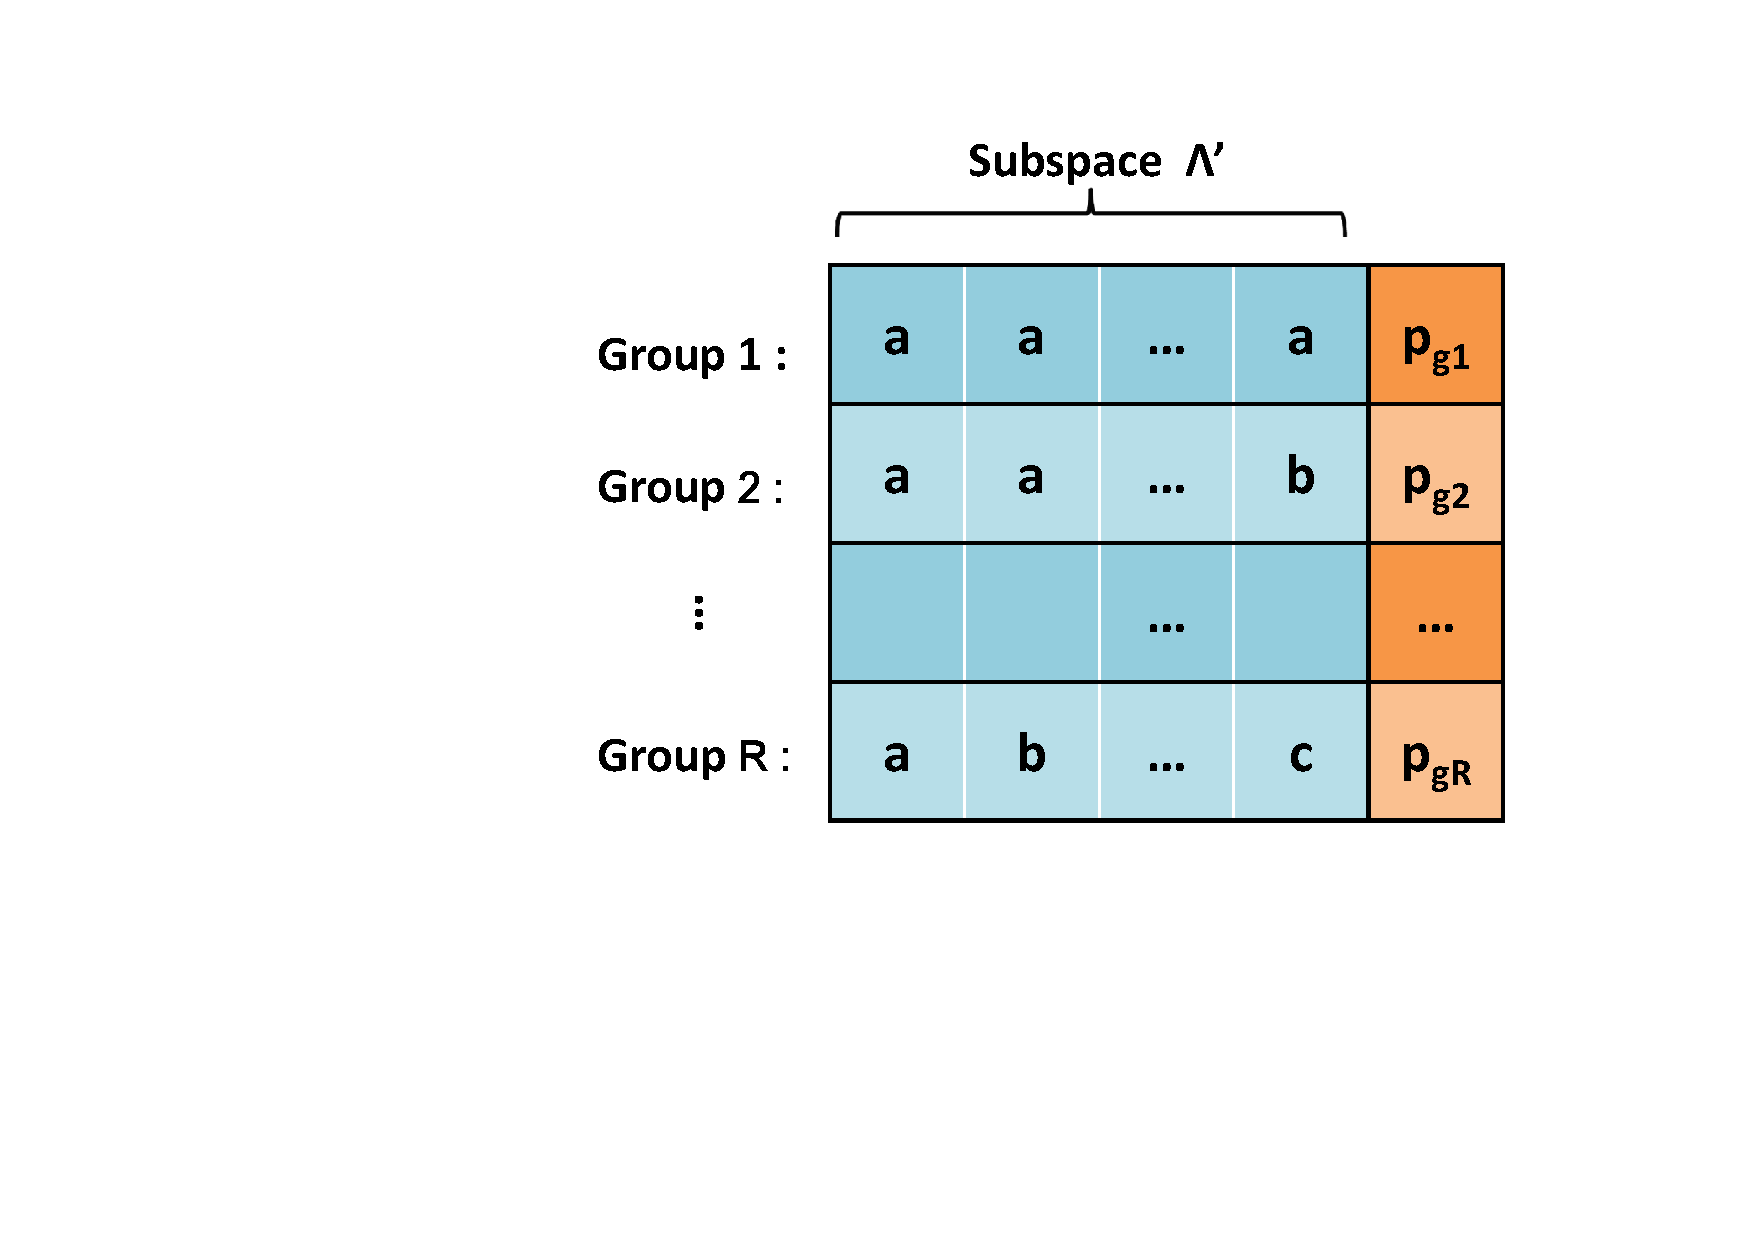
\includegraphics[width = 0.6\columnwidth]{figure/codebook.pdf}
\vspace{-3mm}
\caption{The codebook of an attribute matrix}
\label{fig:codebook}
\end{figure}

\noindent \textbf{Coding cost of the non-cluster area $CC(U)$:} The Non-cluster area consists of the elements in the adjacency matrix $A$ and the attributed matrix $F$ that are not contained in $K$ clusters, which are represented as $U_A$ and $U_F$ respectively. Similarly, the coding cost of the non-cluster area $CC(U)$ is the sum of the structural coding cost $CC(U_A)$ and the attributed coding cost $CC(U_F)$, as shown in Eq.(\ref{eq:nc}). 
\begin{equation}
CC(NC) = CC(U_A) + CC(U_F)
\label{eq:nc}
\end{equation}

We consider all elements of the structural non-cluster area $U_A$ entirely and code them with a fixed coding order. The coding cost of the non-cluster area of the structural aspect $CC(U_A)$ can be encoded as shown Eq.\ref{eq:unclusterA}. Here, $p_1(U_A)$ is the number of edges in $U_A$ and $p_0(U_A)$ is the number of no-egdes in $U_A$. Due to the symmetry property of the matrix, $n_{U_A} = \frac{N_{U_A}\cdot(N_{U_A}-1)}{2}$ is equals to half of the elements in the non-cluster area. 
\begin{equation}
CC(U_A)= -n_{U_A}\cdot (p_1(U_A)\cdot \log_2 p_1(U_A) + p_0(U_A) \cdot \log_2 p_0(U_A)).
\label{eq:unclusterA}
\end{equation}

In the non-cluster area of attribute aspect $U_F$, we encode the remaining categories of each attribute one by one. The coding cost $CC(U_F)$ is calculated in Eq.\ref{eq:unclusterF}, where $N_{\lambda_i}$ is the number of categories of attribute $\lambda_i$ that are not assigned to any clusters, and $p_{\theta_j}$ is the probability of an category $\theta_j$ in the remaining elements of the corresponding attribute. 
\begin{equation}
CC(U_F)= -\sum^T_{i=1}\sum^{\theta_j}_{j=1} N_{\lambda_i}\cdot p_{\theta_j}\cdot \log_2 p_{\theta_j} .
\label{eq:unclusterF}
\end{equation}

\subsubsection{Model Cost $L(M)$}
\noindent For encoding the model cost $L(M)$ of the attributed graph, every cluster will be compressed in three aspects: the assignments of each vertex , the  assignments of each attribute and the parameters of the clusters.
\\

\noindent \textbf{Coding cost of vertices assignment $CC_{IDV}(C_i)$: } As overlapping is allowed in our proposed algorithm, a vertex can be assigned to multiple clusters. For each cluster, we adopt an assignment list to label the existence of vertices. An example for this is shown in Figure \ref{fig:list}. When the vertex belongs to the cluster, the corresponding value in the list is set to $``1"$, otherwise set to $``0"$. Therefore, the coding cost of the vertices assignment for a cluster $CC_{IDV}(C_i)$ is lower bounded by its entropy as shown in Eq.(\ref{eq:nodeid}), where $p_{1}(L)$ and $p_{0}(L)$ denote the probability of $1$ and $0$ in the assignment list of cluster $C_i$ respectively, and $N$ is the number of vertices in the graph. Then the coding cost of the vertice assignments of the whole graph is the sum of cost for all clusters.
\begin{equation}
CC_{IDV}(C_i)= - N \cdot ( p_{1}(L) \cdot \log_2 {p_{1}(L)} +  p_{0}(L) \cdot \log_2 {p_{0}(L)}).
\label{eq:nodeid}
\end{equation}

\begin{figure}[h]
\centering
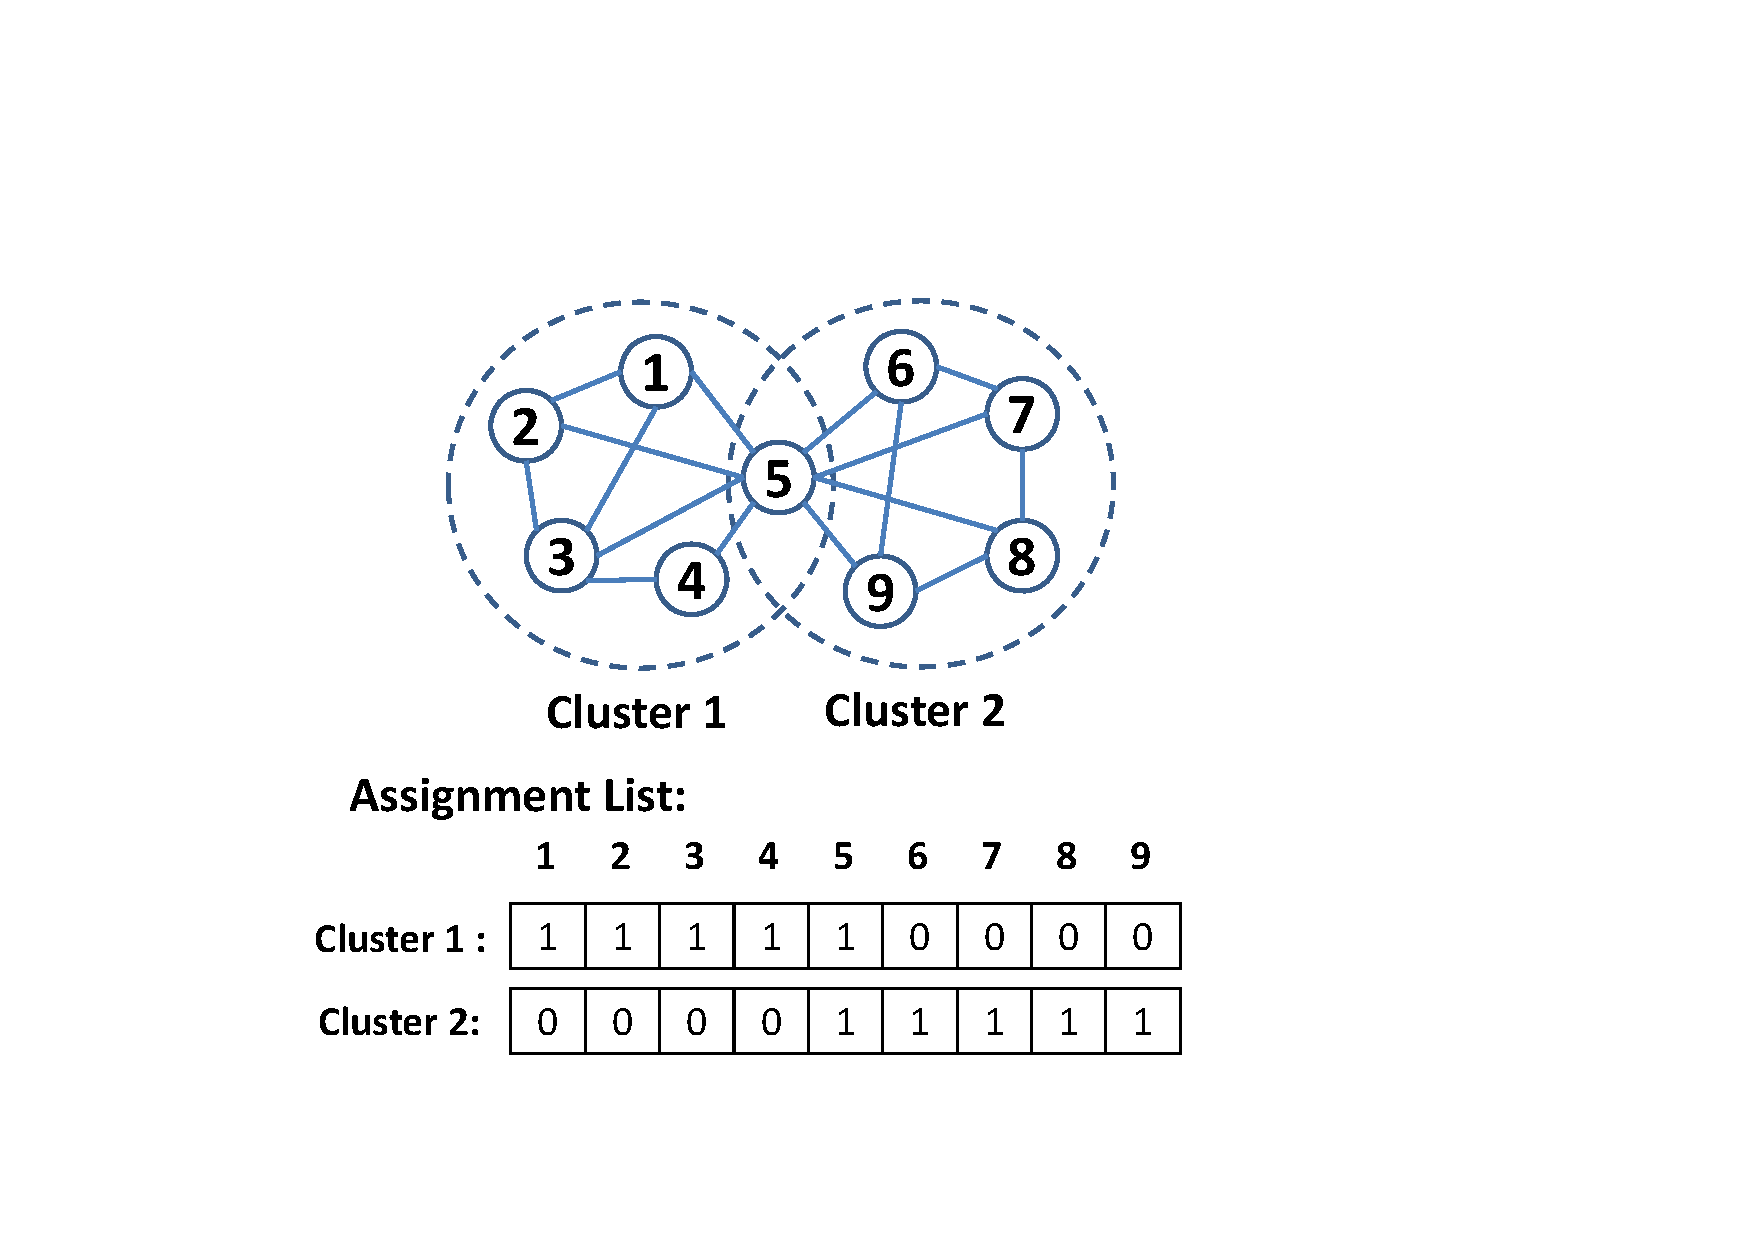
\includegraphics[width = 0.7\columnwidth]{figure/list.pdf}
\vspace{-3mm}
\caption{The assignment list of vertices}
\label{fig:list}
\end{figure}

\noindent \textbf{Coding cost of attributes assignments $CC_{IDF}(C_i)$: }
In our proposed algorithm, the corresponding attribute subspaces of clusters are also detected. Similarly, there is overlapping among the subspaces as well, which means an attribute can be grouped into multiple clusters. Here we also adopt an assignment list with size $T$ to represent attributes that are contained in a subspace of a cluster, which is shown in Eq.(\ref{eq:featureid}).
\begin{equation}
CC_{IDF}(C_i)= - T \cdot ( p_{1}(L) \cdot \log_2 {p_{1}(L)} + p_{0}(L) \cdot \log_2 {p_{0}(L)}).
\label{eq:featureid}
\end{equation}

\noindent \textbf{Coding cost of parameters:} To ensure that the receiver acquires the complete information, all parameters need to be encoded to keep the lossless compression. The cost of these parameters can be calculated from Eq.(\ref{eq:nodepara}), where $n_p$ is the number of parameter and $n_E$ is the number of entries. 
\begin{equation}
CC_{para}= 0.5 \cdot n_p \cdot \log_2 n_E.
\label{eq:nodepara}
\end{equation}

First, we need to encode the probability of $``1"$s and $``0"$s in each cluster $C_i$ and of the non-cluster area $U$. Here $n_p = K + 1$ and $n_E$ is equals to half of the entries of the corresponding subset adjacency matrix $A_{C_i}$. Secondly, we encode he probabilities of  the $R$ groups in the codebook. Here $n_p = R-1$ and $n_E$ are equals to the number of categories of the codebook. Thirdly, in the non-cluster area of the attribute matrix, we encode the probabilities of all categories in each attribute as parameter, for each attribute $i$. For this $n_p = \theta_j -1$ and $n_E$ are equals to the size of the remaining categories of attribute $i$. Finally, we encode the probabilities of the assignment lists as parameters as well, here $n_p = 1$ and $n_E$ are equals to the size of the list. 

%\subsubsection{Cost of Adjacency Matrix $A$}



%The adjacency matrix $A$ embodies structural information with $1$ and $0$ denoting the existence of edges. Suppose $K$ clusters $C=\{C_1,C_2,...,C_K \}$ are discovered from an attributed graph $G$. Then for every cluster in $C$ we need to encode all vertices that are included in that cluster, more specifically we encode the cluster ID the vertices belong to in $CC^A_{ID}$. For doing so we adopt an assignment list with size $N$ to label the existence of vertices in every cluster. When the vertex belongs to a cluster , the corresponding value in the list is set to $1$, or set to $0$. Therefore, the coding cost for the cluster ID of vertices in a cluster $C_i$ is lower bounded by its entropy as shown in Eq.\ref{eq:nodeid}  where $P_{ID}(1)$ in the assignment list of $C_i$ denotes the probability of $1$ while $P_{ID}(0)$ denotes the probability of $0$.
%\begin{equation}
%CC^A_{ID}(C_i)= N \cdot (P_{ID}(1) \cdot log_2 \frac{1}{P_{ID}(1)} + P_{ID}(0) \cdot log_2 \frac{1}{P_{ID}(0)}).
%\label{eq:nodeid}
%\end{equation}
%
%Eq.\ref{eq:clusterA} shows the coding cost of the structural information of each cluster $C_i$, where $P(1)$ and $P(0)$ stands for the probability if a $1$ and respectively a $0$ is standing in the adjacency matrix of cluster $C_i$. $n_{C_i}=\frac{N_{C_i}(N_{C_i}-1)}{2}$ is the number of entries in cluster $C_i$.
%
%\begin{equation}
%CC^A(C_i)= n_{C_i}\cdot (P(1)\cdot log_2 \frac{1}{P(1)} + P(0)\cdot log_2 \frac{1}{P(0)}).
%\label{eq:clusterA}
%\end{equation}
%
%To ensure that the receiver of the compression is acquiring the complete information, all probabilities of the occurrence of $1$ and $0$ in each cluster $C_i$ need to be encoded as two parameters. The cost of these parameters can be calculated from Eq.\ref{eq:nodepara}, where $n_p$ is number of parameter of Cluster $C_i$ and $n_E$ is the number of entries. In cluster $C_i$, $n_E=\frac{N_{C_i}(N_{C_i}-1)}{2}$ is the number of entries, $n_p =2$.
%\begin{equation}
%CC^A_p(C_i)= \frac{n_p-1}{2} \cdot log_2 n_E.
%\label{eq:nodepara}
%\end{equation}
%
%After $K$ clusters are generated by IROC, no-cluster area is consist of all elements in the adjacency matrix $A$ which are not contained in $K$ clusters.. We consider it as an ensemble and calculate its edge probability to receive a loseless compression. Therefore, we need to encode the no-cluster area $U_A$ as in Eq.\ref{eq:unclusterA}, where $P_{U_A}(1)$ is the number of links in $U_A$ and $P_{U_A}(0)$ is the number of disconnection in $U_A$, $n_{U_A} = \frac{N_{U^A}(N_{U^A}-1)}{2}$ is the number of elements in the no-cluster area. Similarly, the parameter costs $CC_p(U_A)$ of $P_{U_A}(1)$ and $P_{U_A}(0)$ can be calculated from Eq.\ref{eq:nodepara}. Again, $n_E = n_{U_A}$ is number of entries in $U_A$ and $n_p = 2$.
%\begin{equation}
%CC(U_A)=n_{U_A}\cdot (P_{U_A}(1)\cdot log_2 \frac{1}{P_{U_A}(1)} + P_{U_A}(0) \cdot log_2 \frac{1}{P_{U_A}(0)}).
%\label{eq:unclusterA}
%\end{equation}
%By all accounts, the coding cost of the adjacency matrix $A$ is exhibited in Eq.\ref{eq:adjcc}.
%
%\begin{equation}
%\begin{split}
%CC^A = \sum_{i=1}^K (CC^A_{ID}(C_i) + CC^A_p(C_i) + CC^A(C_i)) \\+ CC(U_A) + CC_p(U_A).
%\end{split}
%\label{eq:adjcc}
%\end{equation}
%
%
%%\subsubsection{Cost of an Attribute Matrix $F$}
%From the attribute matrix $F$ we are not only obtaining information about the node clusters, but also about the subspace of attributes of each cluster. Because the information of node clusters has already been encoded in the adjacency matrix, only the information of the attributes needs to be encoded in the attributed matrix. Figure \ref{fig:codebook} describes a codebook of an attributed matrix with the cluster $C_i$. $\Lambda'$ being the attribute subspace in which the subset of attributes is $\Lambda$. Every vertex possesses a category in each attribute of the subspace. Equally, in cluster $C_i$, the attributes of a vertex are a category string with a size equal to the subspace. Suppose attribute of $N_{C_i}$ vertex can be formed into $R$ groups and the percentages of each group in a cluster can be calculated as $P_{F1},P_{F2},...,P_{FR}$. Then the information of the attributes of cluster $C_i$ can be encoded as Eq.\ref{eq:clusterF}.
%\begin{figure}[h]
%\centering
%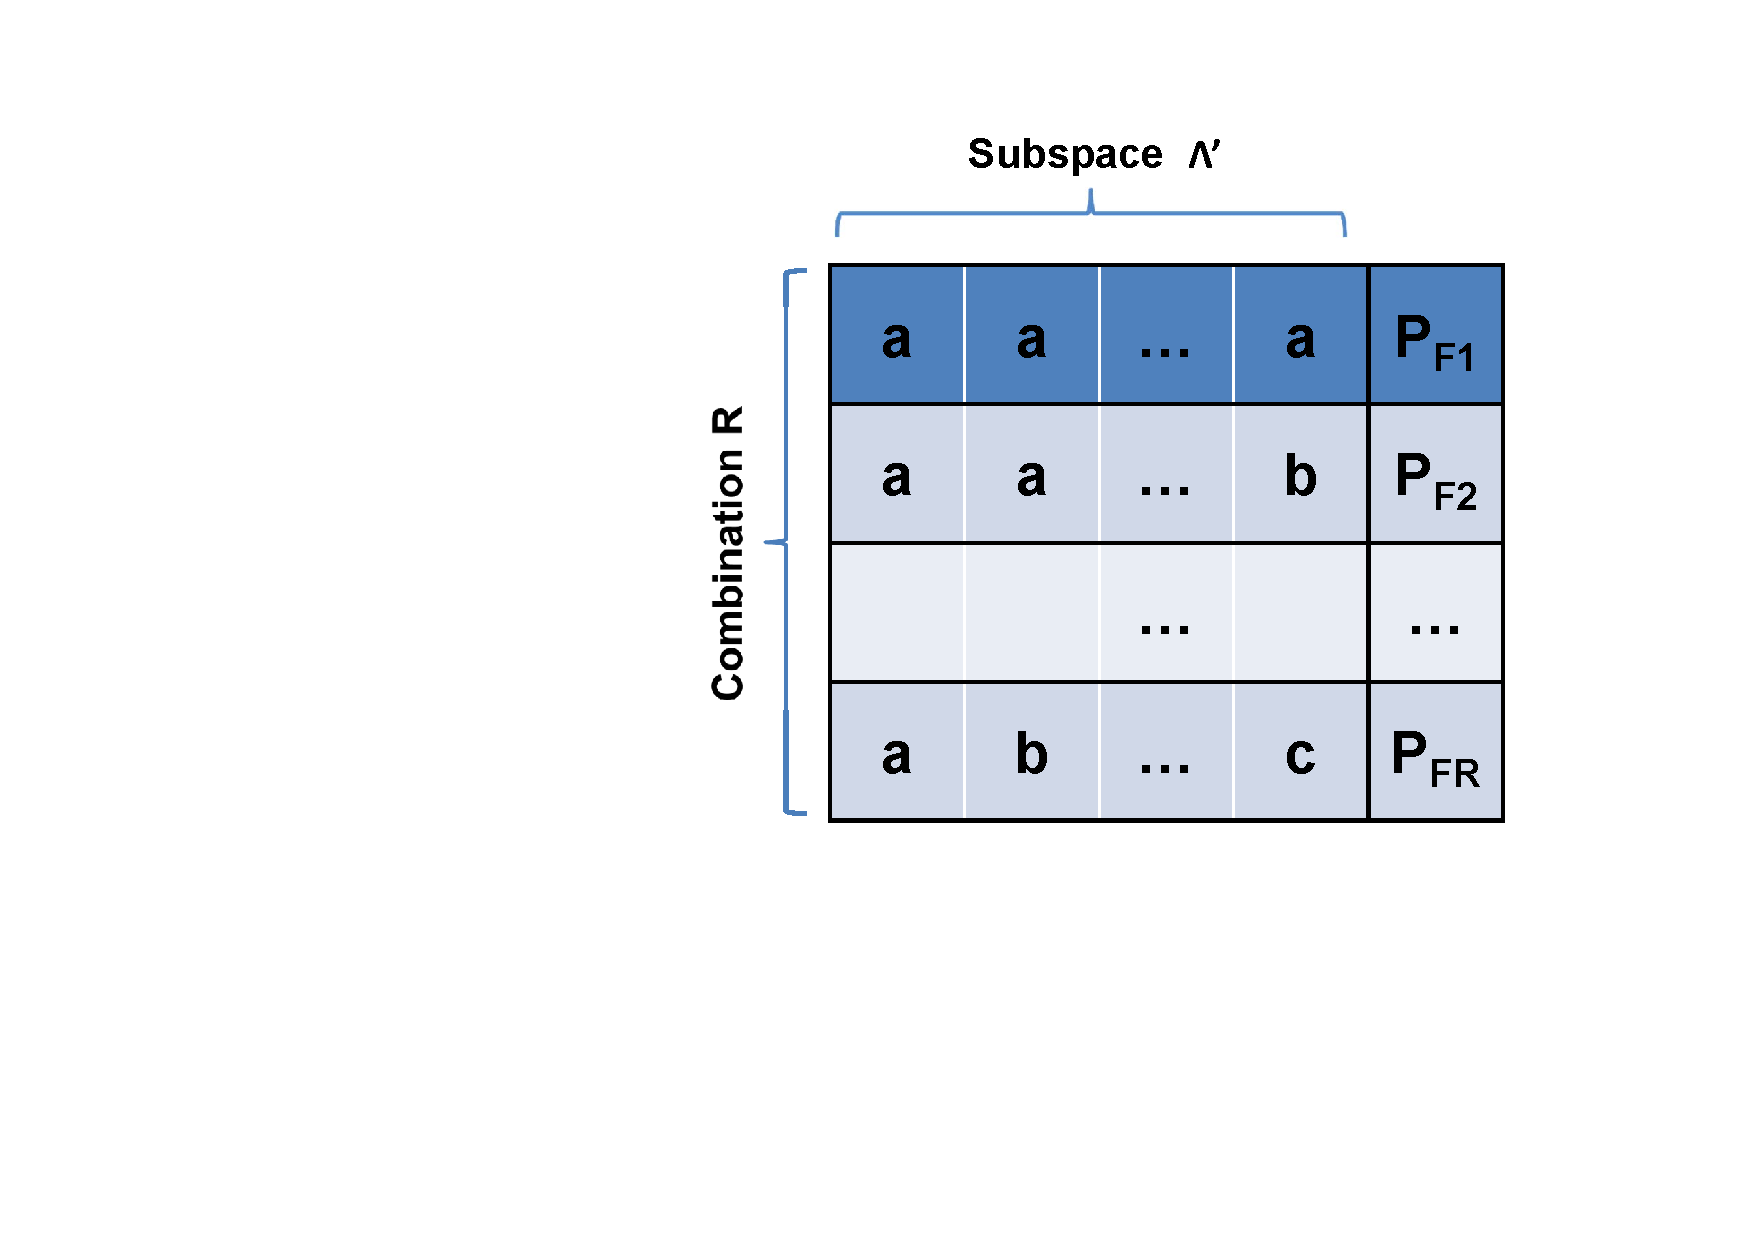
\includegraphics[width = 0.5\columnwidth]{figure/codebooka.pdf}
%\vspace{-3mm}
%\caption{The code book of an attribute matrix}
%\label{fig:codebook}
%\end{figure}
%
%\begin{equation}
%CC^F(C_i)= R \cdot \sum_{i=1}^R P_{Fi}\cdot log_2 \frac{1}{P_{Fi}}
%\label{eq:clusterF}
%\end{equation}
%
%Moreover, the probabilities of a group are encoded as parameter with the cost being calculated from Eq.\ref{eq:nodepara}, where the number of parameters $n_p$ is $R$, and $n_E$ is the number of vertex in cluster $C_i$. Additionally, we use $log_2 \theta_k$ bits to encode a category in a attribute $\lambda_k$. The parameter costs $CC^F_p(C_i)$ of an attribute matrix of a cluster $C_i$ is calculated as is shown in Eq.\ref{eq:Fpara}.
%
%\begin{equation}
%CC^F_p(C_i)= \frac{R -1}{2} \cdot  log_2 N_{C_i} + N_{C_i} \cdot \sum_{i=1}^S log_2 \theta_k.
%\label{eq:Fpara}
%\end{equation}
%
%Similarly, there is also overlapping among the subspaces of clusters. Therefore, we adopt a list with size $ T $ to represent attributes which are contained in a subspace of a cluster.  If the subspace of a cluster includes the attribute, the corresponding value of the list is set as $1$, or set as $0$. Also, the coding cost of the subspace ID of a cluster  $CC^F_{ID}(C_i)$ is calculated from Eq.\ref{eq:featureid}, where $P_S(1)$ denotes in the list of $C_i$ the probability of $1$ which means the attribute is contained in the subspace , and $P_S(0)$ denotes the probability that this attribute is not contained in the subspace -therefore its value is $0$.
%
%\begin{equation}
%CC^F_{ID}(C_i)= T \cdot (P_S(1) \cdot log_2 \frac{1}{P_S(1)} + P_S(0) \cdot log_2 \frac{1}{P_S(0)}).
%\label{eq:featureid}
%\end{equation}
%%
%%and,
%%
%%\begin{equation}
%%\small
%% CC^F' =
%%\label{eq:featureid}
%%\end{equation}
%
%In addition, the no-cluster areas of the attribute matrix are categories of each attribute which are not contained in the clusters. Therefore, we again encode the remaining categories of each cluster for loseless compression as shown in Eq.\ref{eq:unclusterF}, where $N_{\lambda_i}$ is the number of categories of attribute $\lambda_i$ which are not assigned to clusters, and $P_{U_F}(\theta_j)$ is the probability of each category occupied in the remaining elements. Each attribute contains the remaining probabilities of a category, and these probabilities are encoded as parameters which can be calculated from Eq.\ref{eq:unodepara}.
%\begin{equation}
%CC(U_F)= \sum^T_{i=1}\sum^{\theta_j}_{j=1} N_{\lambda_i}\cdot P_{U_F}(\theta_j) \cdot log_2 \frac{1}{P_{U_F}(\theta_j)} .
%\label{eq:unclusterF}
%\end{equation}
%
%\begin{equation}
%CC^F_p(U_F)= \sum^T_{i=1} \frac{\theta_i -1}{2} \cdot log_2 N_{\lambda_i}.
%\label{eq:unodepara}
%\end{equation}
%
%Consequently, the cost of an attribute matrix $F$ is shown in Eq.\ref{eq:attributecc}. Overall the coding cost of an attributed graph $G$ is the sum of costs of the adjacency matrix and the attributed matrix as can be seen in Eq.\ref{eq:cc}.
%\begin{equation}
%\begin{split}
%CC^F = \sum_{i=1}^K (CC^F_{ID}(C_i) + CC^F_p(C_i) + CC^F(C_i))\\
% + CC(U_F) + CC_p(U_F).
%\end{split}
%\label{eq:attributecc}
%\end{equation}
%With that the overall cost can be calculated:
%\begin{equation}
%CC = CC^A + CC^F.
%\label{eq:cc}
%\end{equation}




